\documentclass[11pt]{article}
\usepackage[utf8]{inputenc}
\usepackage{amsmath}
\usepackage{amsfonts}
\usepackage[margin=1in]{geometry}
\usepackage{framed}
\usepackage{tikz}
\usepackage{listings}
\usepackage{graphicx}
\usepackage{bbm}
\usepackage{amsthm}
\newtheorem{theorem}{Theorem}
\newtheorem{corollary}{Corollary}[theorem]
\newtheorem{lemma}{Lemma}[theorem]
\newtheorem{assumption}{Assumption}[theorem]
\newtheorem*{remark}{Remark}
\usepackage{amssymb}
\usepackage{mathrsfs}
\usepackage{amsthm}

\usepackage{mathtools}
%\pagenumbering{gobble}
\newcommand{\maxl}{\lambda}
\newcommand{\vlen}{\boldsymbol{h}}
\newcommand{\vint}{\boldsymbol{\omega}}
\newcommand{\vpla}{\boldsymbol{a}}
\newcommand{\innerone}{D_{11}}
\newcommand{\inneronej}{D_{11j}}
\newcommand{\innertwo}{D_{12}}
\newcommand{\innertwoj}{D_{12j}} 
\newcommand{\innerthree}{D_{22}}
\newcommand{\biasone}{B_1}
\newcommand{\biastwo}{B_2}
\newcommand{\biasthree}{B_3}
\newcommand{\Imn}{D}
\newcommand{\Tmn}{T}
\newcommand{\io}{\mathscr{Q}_{p,q}}
\newcommand{\slle}{\hat{\mu}^{LL}_{0j}}
\linespread{1}
\usepackage{bbold}
\usepackage[utf8]{inputenc}
\usepackage{dirtytalk}
\usepackage{float}

\newcommand{\bigCI}{\mathrel{\text{\scalebox{1.07}{$\perp\mkern-10mu\perp$}}}}
%\usepackage{cite}
%\usepackage[backend=bibtex,style=verbose-trad2]{biblatex}
%\bibliography{lesson7a1} 
%\bibliographystyle{ieeetr}

\DeclareMathOperator*{\argmin}{arg\,min}
\DeclareUnicodeCharacter{2014}{\dash}
\usepackage{hyperref}
%\usepackage{natbib}
\usepackage{url}

\usepackage[numbers]{natbib}
\bibliographystyle{plainnat} 

%\usepackage{biblatex}
%\addbibresource{prelim.bib}

%\bibliographystyle{plain}

%\DeclareUnicodeCharacter{0027}{\dash}
%\DeclareRobustCommand\dash{%
%  \unskip\nobreak\thinspace\textemdash\allowbreak\thinspace\ignorespaces}
%\bibliography{prelim} 
%\pagestyle{headings}
\allowdisplaybreaks
\newcommand{\Var}{\textrm{Var}}
\newcommand{\Cov}{\textrm{Cov}}
\newcommand{\Br}{\mathcal{B}(\mathbb{R})}

 \title{Teaching Statement}
 \author{}
% %\date{Committee Members: Tailen Hsing, Kerby Shedden, Stilian Stoev}
% \date{April 24, 2019}

\begin{document}




\section{Multivariate Model for scores}

Given a model for $Y$, the above gives a relevant functional model. We consider the problem here on how to model the scores $Y$. 

Following Stilian?s formulation, when $d=1$ and $s$ and $t$ are scalar, we consider \begin{align*}
Y(t) &= \int_\mathbb{R}e^{itx}((1 + ix)^{-\nu - 1/2} A1_{\{x > 0\}} + (1 + ix)^{-\nu - 1/2} \overline{A}1_{\{x < 0\}}\tilde{B} (dx)
\end{align*}where $\tilde{B}(dx)$ is $\mathbb{C}^k$-valued Brownian motion with \begin{align*}
\tilde{B}(x) &= \overline{\tilde{B}(-x)} &  \mathbb{E}[\tilde{B}(dx) \tilde{B}(dx)^*] &= \mathbb{I}_k dx
\end{align*}and $A$ is a complex-valued matrix. When $\nu = \nu \mathbb{I}_k$ is a scalar, this above integral gives the covariance \begin{align*}
\mathbb{E}[ Y(t) Y(s)^\top ] &= \int_{\mathbb{R}} e^{i(s-t)x}(1+x^2)^{-\nu-1/2}(AA^*1_{\{x >0\}} + \overline{AA}^*1_{\{x < 0\}})dx.
\end{align*}

\section{Simple Model}

We consider a more simple model and aim to derive its validity for any dimension $d$. In particular, we let $AA^*$ be a constant matrix. Also, specify a hyperplane that goes through the origin in $d-1$ dimensions that is the plane of reflection of the nonreversibility. When a vector lies on the hyperplane, the model is reversible; when one lies perpendicular to the hyperplane, the model is at its most nonreversible direction. This formulation is considerably less flexible than the model described above with $\sigma(\theta)$ and $AA^\star(\theta)$.

\subsection{Formulation for general $d$}

Let $ \vlen, \vint$ be vectors in $\mathbb{R}^d$, and let $AA^* = R + iM$ where $R$ is a $k\times k$ real positive definite matrix and $M = \begin{pmatrix} 0 & -m\\  m & 0\end{pmatrix}$ for some $m \in \mathbb{R}$. Let $\vpla$ be a vector in $\mathbb{R}^d$ that describes the plane through the origin for which the non-reversibility is reflected, defined by all $\vint$ such that $\vpla^\top \vint = 0$.

We want to consider the covariance of \begin{align*}
C(\boldsymbol{0}, \boldsymbol{h}) &= \int_{\mathbb{R}^d} e^{i \vint^\top \vlen} (1 +\vint^\top \vint )^{-\nu- \frac{d}{2}} \left(AA^* 1_{\{\vpla^\top \vint > 0\}} + \overline{AA^*} 1_{\{\vpla^\top\vint < 0\}}\right) d\vint% \\
%&=\int_{\mathbb{R}^d} e^{i \vint^\top \vlen }(1 + \vint^\top \vint)^{-\nu- \frac{d}{2}} \left((R + iM)1_{\{\vpla^\top\vint > 0\}} + (R - iM) 1_{\{\vpla^\top\vint < 0\}}\right) d\vint 
\end{align*}
Plugging in $AA^* = R + iM$ gives
\begin{align*}
C(\boldsymbol{0}, \boldsymbol{h})&=\int_{\mathbb{R}^d} e^{i \vint^\top \boldsymbol{h}}(1 + \vint^\top \vint)^{-\nu- \frac{d}{2}} \left(R + iM1_{\{\vpla^\top\vint > 0\}}  - iM1_{\{\vpla^\top\vint < 0\}}\right) d\vint\end{align*}
and by breaking up the integral we have
\begin{align*}
C(\boldsymbol{0}, \boldsymbol{h})%&=\int_{\mathbb{R}^d} (\cos(\vint^\top \boldsymbol{h}) + i\sin(\vint^\top \boldsymbol{h}))(1 + \vint^\top \vint)^{-\nu- \frac{d}{2}} \left(R + iM1_{\{\vint > 0\}}  - iM1_{\{\vint < 0\}}\right) d\vint \\
&=\int_{\mathbb{R}^d}\cos(\vint^\top \boldsymbol{h})(1 + \vint^\top \vint)^{-\nu- \frac{d}{2}} \left(R + iM1_{\{\vpla^\top\vint > 0\}}  - iM1_{\{\vpla^\top\vint < 0\}}\right) d\vint \\
&\ \ \ \ \ \ +i\int_{\mathbb{R}^d}\sin(\vint^\top \boldsymbol{h})(1 + \vint^\top \vint)^{-\nu- \frac{d}{2}} \left(R + iM1_{\{\vpla^\top\vint > 0\}}  - iM1_{\{\vpla^\top\vint < 0\}}\right) d\vint.\end{align*}
Using the even and odd properties of the cosine and sine functions, respectively, gives
\begin{align*}
C(\boldsymbol{0}, \boldsymbol{h})&=R\int_{\mathbb{R}^d}\cos(\vint^\top \boldsymbol{h})(1 + \vint^\top \vint)^{-\nu- \frac{d}{2}} d\vint \\
& \ \ \ \ \ + i^2M\int_{\mathbb{R}^d}\sin(\vint^\top \boldsymbol{h})(1 + \vint^\top \vint)^{-\nu- \frac{d}{2}} \left(1_{\{\vpla^\top\vint > 0\}}  - 1_{\{\vpla^\top\vint < 0\}}\right) d\vint \\
&=R\int_{\mathbb{R}^d}\cos(\vint^\top \boldsymbol{h})(1 + \vint^\top \vint)^{-\nu- \frac{d}{2}} d\vint \\
& \ \ \ \ \ -2M\int_{\vint | \vpla^\top\vint > 0}\sin(\vint^\top \boldsymbol{h})(1 + \vint^\top \vint)^{-\nu- \frac{d}{2}} d\vint .%&\ \ \ \ \ +i\int_{\mathbb{R}^d} e^{i \vint^\top \boldsymbol{h}}(1 + \vint^\top \vint)^{-\nu+ \frac{d}{2}} \left( F(\vint)1_{\{\vint > 0\}}  - F(\vint)1_{\{\vint < 0\}}\right) d\vint 
\end{align*}%by using the even and odd properties of the cosine and sine functions, respectively.

When $M$ is the $0$ matrix, each component is Matern, and the above is a simplified version of Gneiting et al (2010) with scale parameter $1$, which is a valid covariance iff $R$ is positive definite and $\nu > 0$. The derivation of the Matern covariance in the univariate case in arbitrary dimension is given in Stein 1999 \textit{Interpolation of Spatial Data}.



 Therefore, in the following, we focus on evaluating the second integral: \begin{align}
\int_{\vint | \vpla^\top\vint > 0}\sin(\vint^\top \boldsymbol{h})(1 + \vint^\top \vint)^{-\nu- \frac{d}{2}} d\vint \label{toughintegral}
\end{align}

%Focusing on the second part, and letting $r = \left\lVert \vint \right\rVert$ we have \begin{align*}
%&-2M\int_{\mathbb{R}^{d-1} \times \mathbb{R}^+}\sin(\vint^\top \boldsymbol{h})(1 + \vint^\top \vint)^{-\nu- \frac{d}{2}} d\vint \\
%&= -2M \int_{S^{d-1}} \int_0^\infty\sin(r\thet\vpla \boldsymbol{h})(1 + r^2)^{-\nu- \frac{d}{2}} drd\theta \\
%&= -2M \int_{S^{d-1}} (I_{\nu}\theta \\
% \end{align*}
% 

\subsection{$d=1$}
 Consider the case $d=1$ where $\omega$ and $h$ are scalars and we have 
  \begin{align*}
&\int_{\omega > 0}\sin(\omega h)(1 + \omega^2)^{-\nu- \frac{1}{2}} d\omega \\
&= \textrm{sign}(h) |h|^{\nu} 2^{-\nu-1} \sqrt{\pi} \Gamma(-\nu + 1/2)\left(I_{\nu}(|h|) - \boldsymbol{L}_{-\nu} (|h|)\right)
 \end{align*}given on page 332 of Watson: \textit{Theory of Bessel Functions} and $I_\nu$ is the modified Bessel function and $\boldsymbol{L}_\nu$ is the modified Struve function. Note that the above is undefined for $\nu = 1/2, 3/2, \dots$ due to the gamma function, where we have extended the gamma function to the negative nonintegers. \fbox{What happens when $\nu = 1/2, 3/2, \dots$?}
 
 \subsection{$d=2$}
 
%Consider the case $d$ dimensional case% and note that $$\sin(\vint^\top \boldsymbol{h}) = \sin(r |\boldsymbol{h}| \cos(\theta))$$where $\theta$ is the angle between $\vint$ and $\boldsymbol{h}$.
%  \begin{align*}
%&-2M\int_{\mathbb{R} \times \mathbb{R}^+}\sin(\vint^\top \boldsymbol{h})(1 + \vint^\top \vint)^{-\nu- 1} d\vint \\
%&=-2M \int_0^\pi \int_0^\infty \sin(r\thet\vpla \boldsymbol{h}) (1 + r^2)^{-\nu-1} r drd\theta
%%&=-2M \textrm{sign}(h) |h|^{\nu} 2^{-\nu-1} \sqrt{\pi} \Gamma(-\nu + 1/2)\left(I_{\nu}(|h|) - L_{-\nu} (|h|)\right)
% \end{align*}
 
 For the 2-dimensional case, we switch to polar coordinates. Note that $\sin(\vint^\top \boldsymbol{h}) = \sin(r \left\lVert \boldsymbol{h}\right\rVert \cos(\theta))$ where $\theta$ is the angle between $\vint$ and $\boldsymbol{h}$ and $r = \left\lVert \vint \right\rVert$. Assume these polar coordinates, and let $c$ be the angle that $\boldsymbol{h}$ makes with the $x$ axis. Finally, assume without loss of generality that $a = (0,1)^\top$ so that we integrate over the upper half of $\mathbb{R}^2$. See the figure below for a visual representation. Then the integral (\ref{toughintegral}) is \begin{align*}
&\int_{\vint | \vpla^\top \vint > 0}\sin(\vint^\top \boldsymbol{h})(1 + \vint^\top \vint)^{-\nu- 1} d\vint \\
&= \int_0^\infty  \int_{-\pi + c}^{c} \sin(r\left\lVert \boldsymbol{h}\right\rVert \cos(\theta)) (1 +r^2)^{- \nu - 1} r d\theta dr. %\\ 
%&=-2M \textrm{sign}(h) |h|^{\nu} 2^{-\nu-1} \sqrt{\pi} \Gamma(-\nu + 1/2)\left(I_{\nu}(|h|) - L_{-\nu} (|h|)\right)
 \end{align*}

 
Now, by 12.1.7 of Abramowitz and Stegun \textit{Handbook of Mathematical Functions}, 
\begin{align*}
 \int_0^{\pi/2}  \sin(r\left\lVert \boldsymbol{h}\right\rVert \cos(\theta)) d\theta= \frac{\pi}{2} \boldsymbol{H}_{0}(r\left\lVert \boldsymbol{h}\right\rVert) \end{align*}where $\boldsymbol{H}_\nu$ is the Struve function. One can further see that \begin{align*}
  &\int_{\pi/2}^\pi  \sin(r\left\lVert \boldsymbol{h}\right\rVert \cos(\theta)) d\theta= -\frac{\pi}{2} \boldsymbol{H}_{0}(r\left\lVert \boldsymbol{h}\right\rVert) &   &\int_{-\pi/2}^0  \sin(r\left\lVert \boldsymbol{h}\right\rVert \cos(\theta)) d\theta= \frac{\pi}{2} \boldsymbol{H}_{0}(r\left\lVert \boldsymbol{h}\right\rVert)
 \end{align*}based on properties of $\sin$ and $\cos$. We can now evaluate for two values of $c$:
 
 \begin{enumerate}
\item $c = \pi$: the above integral is $0$, which makes sense since this is the reversible direction as defined. This non-reversible part of the covariance is $0$.
\item $c = \pi/2$: We have \begin{align}
\begin{split} \int_0^\infty  \int_{-\pi/2}^{\pi/2} \sin(r\left\lVert \boldsymbol{h}\right\rVert \cos(\theta)) (1 +r^2)^{- \nu - 1} r d\theta dr&= \int_0^\infty \pi\boldsymbol{H}_0(r\left\lVert \boldsymbol{h}\right\rVert)(1 + r^2)^{-\nu - 1} r dr \\
& =\pi\frac{2^{-\nu -1} \pi \left\lVert \boldsymbol{h}\right\rVert^{\nu}}{\Gamma(\nu+1) \cos(\nu \pi)} \left( I_{\nu }(\left\lVert \boldsymbol{h}\right\rVert) - \boldsymbol{L}_{-\nu} (\left\lVert \boldsymbol{h}\right\rVert)\right)\end{split}\label{complete}
\end{align}by 6.814 of I.S. Gradshteyn and I.M. Ryzhik \textit{Tables of Integrals, Series, and Products}. This gives the non-reversible part perpendicular to the reversible direction. It looks similar to the 1-d case.
 \end{enumerate}
 
 However, this does not work in general because $c\notin \{\pi, \pi/2\}$ necessarily. 


An example of what is going on below. For a fixed $\boldsymbol{h}$, one integrates $\vint$ against the upper half plane. When $\boldsymbol{h}$ is in line with the $x$ axis, the integral is $0$ and the model is reversible across this axis; when $\boldsymbol{h}$ points directly up or down, $c= \pi/2$ and the model is at its most non-reversible direction.

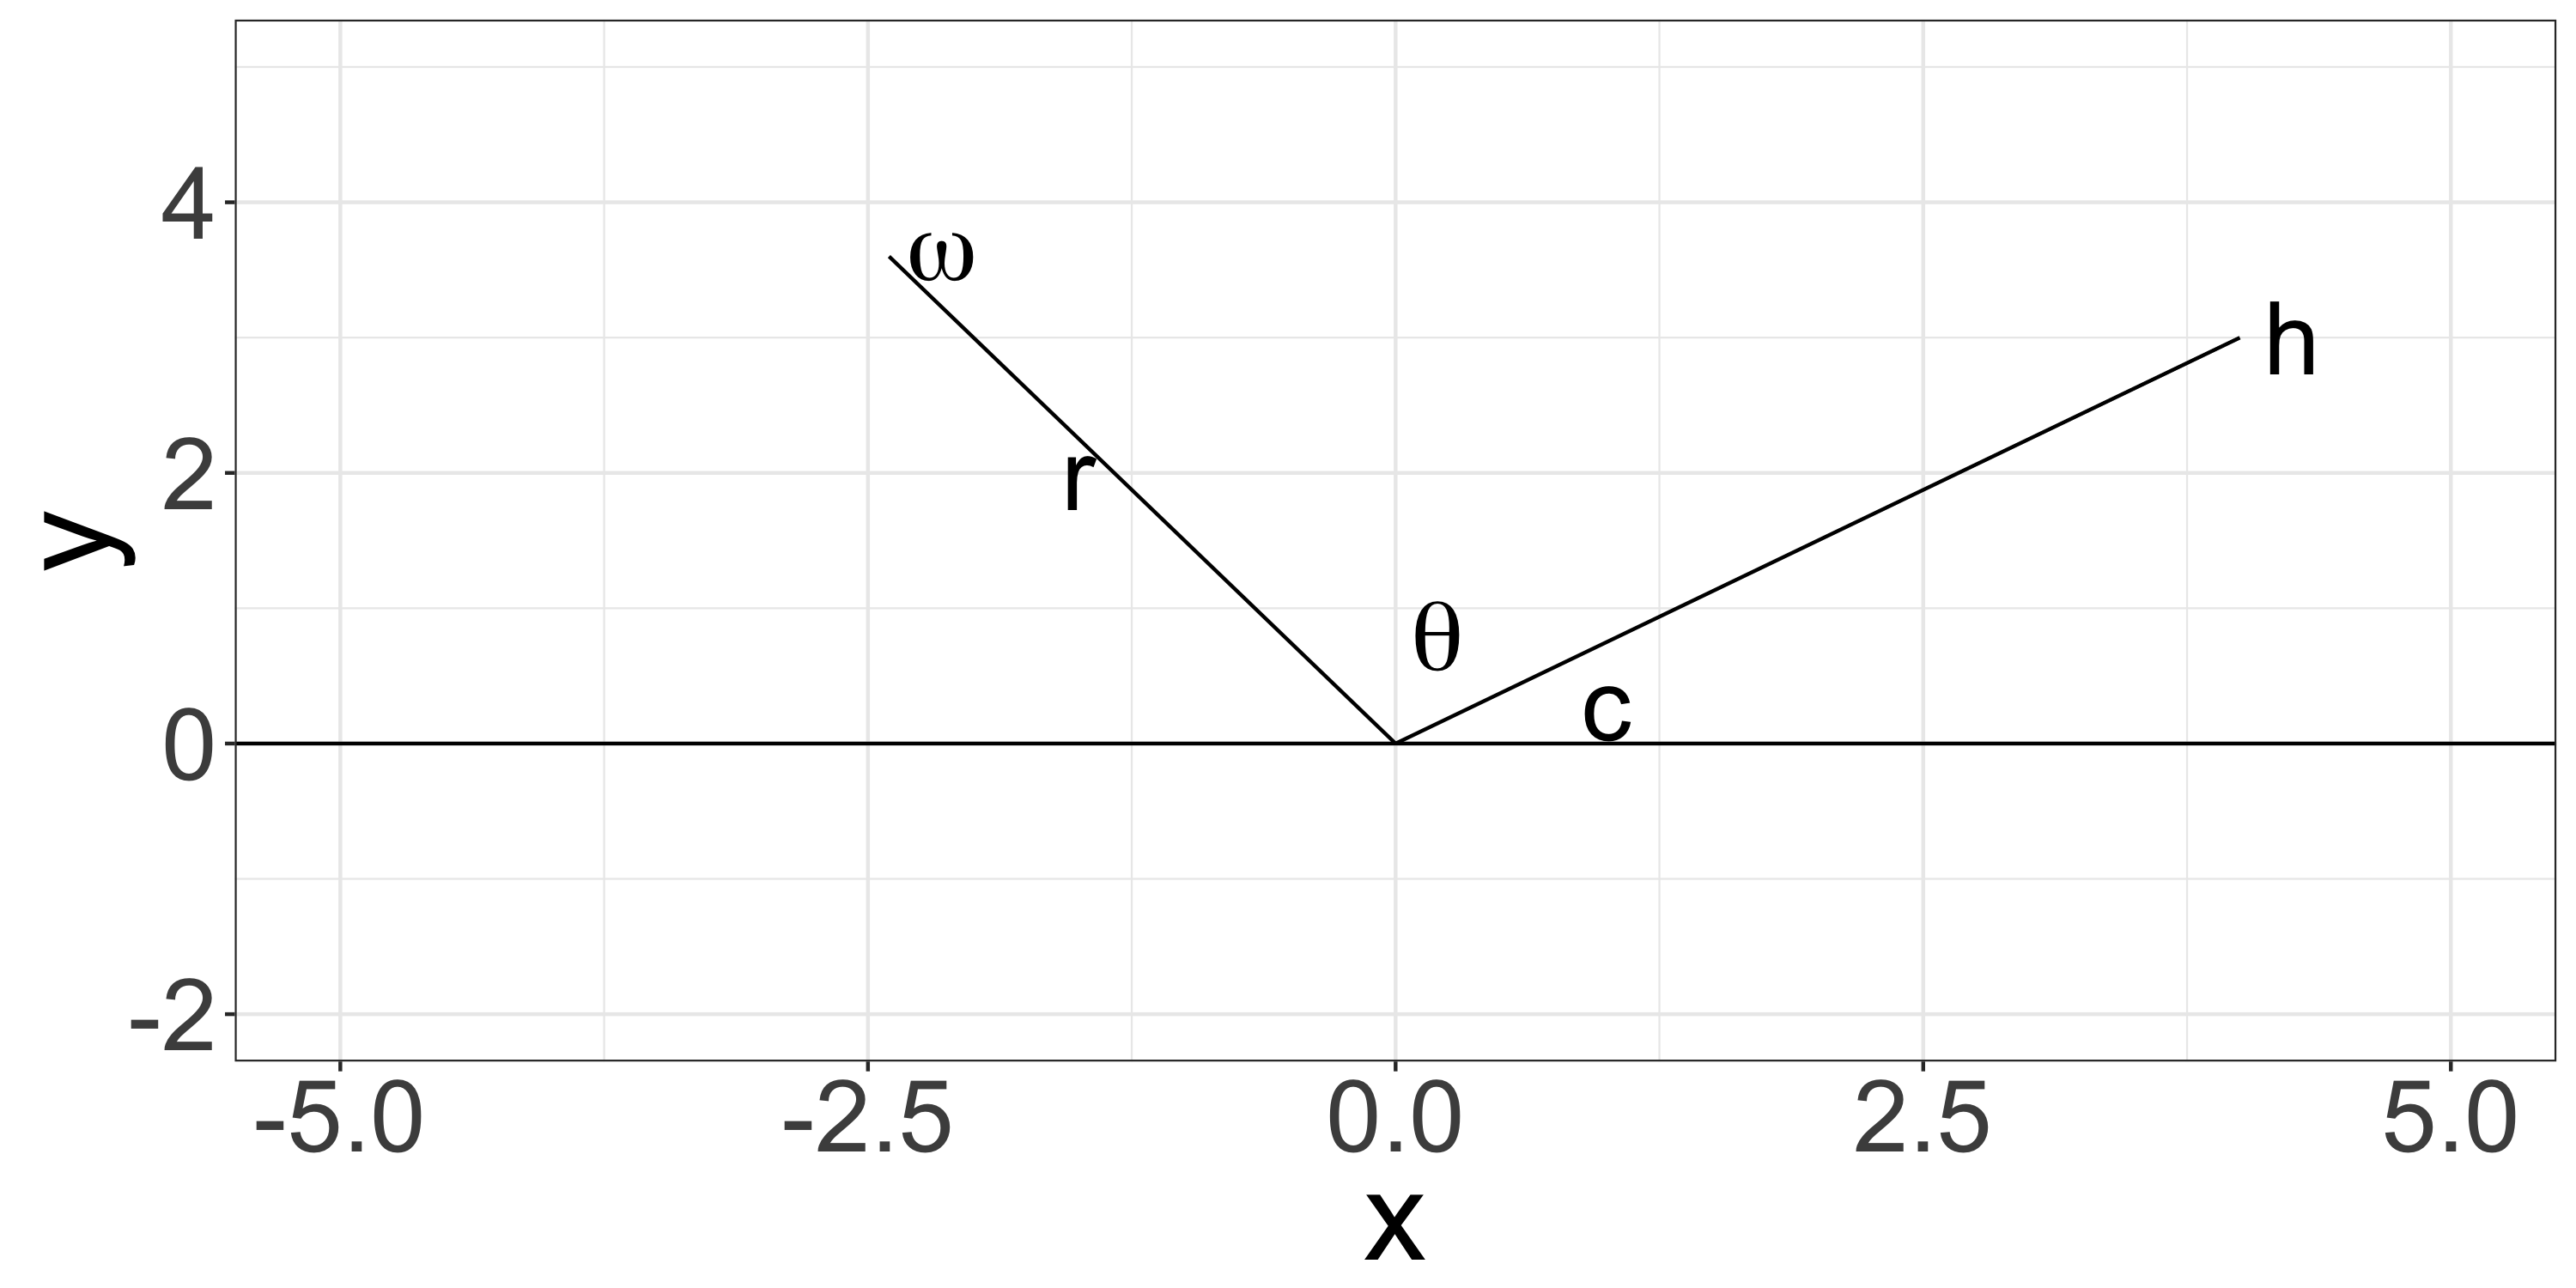
\includegraphics[scale = .1]{angle_plot.png}


 By (1.8) on page 24 of \textit{Theory of incomplete cylindrical functions and their applications} by M. M. Agrest  M. S. Maksimov, we have \begin{align*}
 \int_0^{c}  \sin(r\left\lVert \boldsymbol{h}\right\rVert \cos(\theta)) d\theta= \frac{\pi}{2} \boldsymbol{H}_{0}(c, r\left\lVert \boldsymbol{h}\right\rVert)
 \end{align*}where $\boldsymbol{H}_{\nu}(c, z)$ is the incomplete Struve function. Thus, we are left to evaluate \begin{align*} 
 \int_0^\infty \frac{\pi}{2}\left(\boldsymbol{H}_{0}(c, r\left\lVert \boldsymbol{h}\right\rVert) + \boldsymbol{H}_{0}(\pi - c, r\left\lVert \boldsymbol{h}\right\rVert)\right) (1+r^2)^{-\nu-1} r dr
 \end{align*}
 
% \fbox{What is the value of the integral $\int_0^\infty \boldsymbol{H}_{0}(c, r\left\lVert \boldsymbol{h}\right\rVert) (1 +r^2)^{-\nu - 1} r dr$?}
 
 
By (5.10) on page 183 of \textit{Theory of incomplete cylindrical functions and their applications} and setting $\mu = 2$ and $\nu = 0$, we have $$\int_0^\infty \frac{-\boldsymbol{H}_{0}(c, ax)}{(x^2 + k^2)^{m+1}}x dx = \frac{\pi}{m!} (-1)^{m+1} \left(\frac{d}{dk^2}\right)^{m} F_0^-(c, ak)$$where $$F_0^-(c, ak)=\left\{\frac{I_{0}(c, ak) - \boldsymbol{L}_0(c, ak)}{2}\right\}$$and $I_0(\cdot, \cdot)$ is the incomplete modified Bessel function of the first kind and $\boldsymbol{L}_0(\cdot, \cdot)$ is the incomplete modified Struve function. When $c=  \pi/2$ these reduce to their \say{complete} versions. %This looks close but not exactly right ($m$ is an integer, $\nu$ should be flexible, derivative).

\fbox{\textbf{special case of $\nu=0$}}
Consider the special case where $\nu = 0$. Then, the entire integral is \begin{align*}
&\int_0^\infty\frac{\pi}{2} \left(\boldsymbol{H}_{0}(c, r\left\lVert \boldsymbol{h}\right\rVert) + \boldsymbol{H}_{0}(\pi - c, r\left\lVert \boldsymbol{h}\right\rVert)\right) (1 + r^2)^{-1} r dr \\
\ \ \ \ \ \ \ \ \ &= \frac{\pi}{2} \frac{\pi}{2}\left( I_0(c, \left\lVert \boldsymbol{h}\right\rVert) - \boldsymbol{L}_0(c,\left\lVert \boldsymbol{h}\right\rVert) + I_0(\pi - c, \left\lVert \boldsymbol{h}\right\rVert) - \boldsymbol{L}_0(\pi - c,\left\lVert \boldsymbol{h}\right\rVert)\right)
\end{align*}

When $c = \pi/2$, we reduce to $$\frac{\pi^2}{2} \left( I_0(\left\lVert \boldsymbol{h}\right\rVert) - \boldsymbol{L}_0(\left\lVert \boldsymbol{h}\right\rVert) \right)$$which matches with (\ref{complete}). When $c = \pi$, this reduces to $0$ as expected. 

\fbox{\textbf{different values of $\nu$}}

Assuming that fractional derivatives exist and that we can replace the factorial with the gamma function, we have that , we have \begin{align*}
\int_0^\infty \frac{-\boldsymbol{H}_{0}(c, r \left\lVert \boldsymbol{h}\right\rVert)}{(1 + r^2)^{\nu+1}}r dr=
\frac{\pi}{\Gamma(\nu + 1)} (-1)^{\nu + 1} \left(\frac{d}{d\left\lVert \boldsymbol{h}\right\rVert}\right)^{2\nu} F_0^-(c, \left\lVert \boldsymbol{h}\right\rVert)
\end{align*}I'm not sure how to deal with $(-1)^{\nu + 1}$. Consider $\nu= 1/2$. Then this integral is $$\frac{1}{2} \frac{d}{d \left\lVert \boldsymbol{h}\right\rVert} E_0^+(c,i\left\lVert \boldsymbol{h}\right\rVert)$$which is $$\frac{i}{2} \left(- E_1^+(c,i\left\lVert \boldsymbol{h}\right\rVert) + \frac{2 i \sin(c)}{\pi } e^{i\left\lVert \boldsymbol{h}\right\rVert \cos(c)}\right)$$by using pages 31 and 25. This then becomes $$\frac{i}{2} \left(- 2 e^{i \pi/2}F_1^-(c,\left\lVert \boldsymbol{h}\right\rVert) + \frac{2 i \sin(c)}{\pi } e^{i\left\lVert \boldsymbol{h}\right\rVert \cos(c)}\right)$$ which is $$F_1^-(c,\left\lVert \boldsymbol{h}\right\rVert) - \frac{ \sin(c)}{\pi } e^{i\left\lVert \boldsymbol{h}\right\rVert \cos(c)}$$ which is $$\frac{I_1(c,\left\lVert \boldsymbol{h}\right\rVert) - L_1(c, \left\lVert \boldsymbol{h}\right\rVert)}{2}  - \frac{ \sin(c)}{\pi } e^{i\left\lVert \boldsymbol{h}\right\rVert \cos(c)}$$ 
%Consider $\nu = 1$. Then we must compute \begin{align*}\frac{d}{dk^2} F_0^-(c,ak) &= \frac{d}{dk^2} \frac{1}{2} E_0^+(c, iak) \\
%&= \psi_{1}(c, iz) \frac{A_1}{2\pi iz} i^2 \\ 
%&= (iz E_0^+(w, iz) - E_1^+(w, iz)) \frac{A_1}{2\pi z} i\\
%&=
%\end{align*}
%
%Consider $\nu = 1$. Then we must compute \begin{align*}\frac{d}{dk^2} F_0^-(c,ak) &= \frac{d}{dk^2} \frac{1}{2} E_0^+(c, iak) \\
%&= \psi_{1}(c, iz) \frac{A_1}{2\pi iz} i^2 \\ 
%&= (iz E_0^+(w, iz) - E_1^+(w, iz)) \frac{A_1}{2\pi z} i\\
%&= (iz  F_0^-(w, z) -  e^{i \pi/2}F_1^-(w,z)) \frac{A_1}{\pi z} i \\
%&= (-  F_0^-(w, z) -  \frac{i}{z}e^{i \pi/2}F_1^-(w,z)) \frac{2A_1}{\pi } \\
%&= (-  F_0^-(w, z) +  \frac{1}{z}F_1^-(w,z)) \frac{A_1}{\pi } \\
%\end{align*}


\pagebreak



Now, this derivative can be evaluated using (1.22) on page 25 and (1.37) on page 27 such that \begin{align*}
\left(\frac{d}{dk}\right)^{2m} F_0^-(c,ak) &=\frac{1}{2} \left(\frac{d}{dk}\right)^{2m} E_0^+(c, iak)  \\
&=i^{m} \frac{A_m}{2\pi (ak)^m} \psi_{m}(c, iak)
\end{align*}

Therefore, the entire integral is \begin{align*}
 &\int_0^\infty \frac{\pi}{2}\left(\boldsymbol{H}_{0}(c, r\left\lVert \boldsymbol{h}\right\rVert) - \boldsymbol{H}_{0}(\pi - c, r\left\lVert \boldsymbol{h}\right\rVert)\right) (1+r^2)^{-\nu-1} r dr \\
 &\ \ \ \ \ \ \ \ \ \ \ = \frac{\pi}{\nu!}(-1)^{\nu + 1} i^\nu \frac{A_\nu}{2\pi \left\lVert \boldsymbol{h}\right\rVert^\nu} \left(-\psi_\nu(c, i\left\lVert \boldsymbol{h}\right\rVert) + \psi_\nu(\pi-c, i\left\lVert \boldsymbol{h}\right\rVert)  \right)\\
 &\ \ \ \ \ \ \ \ \ \ \ = \frac{\pi}{\nu!}(-1)^{\nu + 1} i^\nu \frac{A_\nu}{\pi \left\lVert \boldsymbol{h}\right\rVert^\nu} \left(\frac{(i\left\lVert \boldsymbol{h}\right\rVert)^\nu}{A_\nu} \left(-\int_0^c e^{-\left\lVert \boldsymbol{h}\right\rVert \cos (t)} \cos^{2\nu} (t) dt + \int_0^{\pi - c} e^{-\left\lVert \boldsymbol{h}\right\rVert \cos (t)} \cos^{2\nu} (t) dt  \right)\right)\\
 &\ \ \ \ \ \ \ \ \ \ \ = \frac{1}{\nu!} \left(\int_c^{\pi-c} e^{-\left\lVert \boldsymbol{h}\right\rVert \cos (t)} \cos^{2\nu} (t) dt  \right)\\
  &\ \ \ \ \ \ \ \ \ \ \ = \frac{1}{\nu!} \left(\int_c^{\pi-c} e^{-\left\lVert \boldsymbol{h}\right\rVert \cos (t)} \cos^{2\nu} (t) dt  \right)\\
 &\ \ \ \ \ \ \ \ \ \ \ = \frac{-2}{\nu!} \frac{A_\nu}{2\left\lVert \boldsymbol{h}\right\rVert^\nu}  \left(E_\nu^-(c,  \left\lVert \boldsymbol{h}\right\rVert) + E_\nu^-(\pi - c,  \left\lVert \boldsymbol{h}\right\rVert) \right)
 \end{align*}

The first step comes from using hte derivative. . The second step is using the definition of $\phi$. The third step is cancelling and combining integrals. 

USE PAGE 31

By (5.10) on page 183 of \textit{Theory of incomplete cylindrical functions and their applications} and setting $\mu = 2$ and $\nu = 0$, we have $$\int_0^\infty \frac{-\boldsymbol{H}_{0}(c, ax)}{(x^2 + k^2)^{m+1}}x dx = \frac{\pi}{m!} (-1)^{m+1} \left(\frac{d}{dk^2}\right)^{m} F_0^-(c, ak)$$where $$F_0^-(c, ak)=\left\{\frac{I_{0}(c, ak) - \boldsymbol{L}_0(c, ak)}{2}\right\}$$WE NEED AN $i$ in both of theseand $I_0(\cdot, \cdot)$ is the incomplete modified Bessel function orf the first kind and $\boldsymbol{L}_0(\cdot, \cdot)$ is the incomplete modified Struve function. When $m = 0$, this is $$\frac{\pi}{2} (L_0(c, ak) - I_0(c, ak) ).$$ Therefore, the entire integral when $\nu = 0$ is \begin{align*}
 &\int_0^\infty \frac{\pi}{2}\left(\boldsymbol{H}_{0}(c, r\left\lVert \boldsymbol{h}\right\rVert) + \boldsymbol{H}_{0}(\pi - c, r\left\lVert \boldsymbol{h}\right\rVert)\right) (1+r^2)^{-1} r dr \\
 &\ \ \ \ \ \ \ \ \ \ \ = \frac{\pi}{4juhnjjnj} \left(L_0(c, \left\lVert \boldsymbol{h}\right\rVert) - I_0(c, \left\lVert \boldsymbol{h}\right\rVert) + L_0(\pi - c, \left\lVert \boldsymbol{h}\right\rVert) -I_0(\pi - c, \left\lVert \boldsymbol{h}\right\rVert)\right)
 \end{align*}
This, when $c = \pi/2$ matches the formula for (\ref{complete}) where $\nu = 0$.  Similarly, when $c = \pi$, the above is $0$ as expected. This isn't quite right. (no h)









\end{document}